\newpage
\chapter{Demonstration and Evaluation}
After the system's features have been implemented, the system as a result of this research project can be demonstrated and evaluated. This chapter presents a demonstration of the use cases derived from the thesis' goal as well as its evaluation based on the requirements analysis elicited in \autoref{requirements_analysis}.

\section{Demonstration}
Since the extension was originally designed for Marta's website, the demonstration will use it as an example. As a result of this thesis, the following procedure is demonstrated in this chapter:

\begin{enumerate}
  \item With the extension installed, visit any webpage with URL path or query
  \item Store the URL path and query in a JSON format
  \item Reload the page
  \item Open the extension pop-up and see how many times the URL parameters are entered
\end{enumerate}

Since the extension is not published in the Chrome Web Store yet, the \texttt{dist} directory is loaded manually to \verb;chrome://extensions;. After loading the extension, it appears in the Chrome Extensions Toolbar. Opening the extension the first time will notify users that the entries for the specific host is empty (See \autoref{fig:filtreNoEntries}).

\begin{figure}[H]
  \centering
  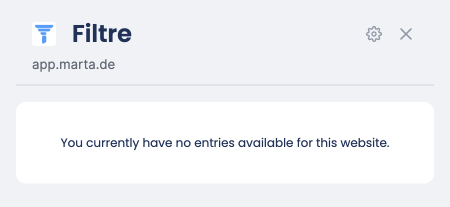
\includegraphics[width=0.7\textwidth]{assets/Filtre_no_entries.png}
  \caption{Screenshot of the no entries available page}
  \label{fig:filtreNoEntries}
\end{figure}

In Marta's webapp, families can find suitable caregivers from the URL \url{app.marta.de/caregivers}. The page restricts the search to 30 caregivers. As a result, in addition to the limitation, a filter based on URL query is implemented, allowing families to filter more caregivers. A modal dialog\footnote{\emph{Modal dialog} is a dialog that appears on top of the main content and moves the system into a special mode requiring user interaction. More information on \url{https://www.nngroup.com/articles/modal-nonmodal-dialog/}} is shown to configure the filter. After adjusting the filter settings, the URL is changed to: \url{app.marta.de/caregivers?caregiver.germanVerbalProficiency=one}. This URL is now stored in the \texttt{chrome.storage} of the extension. \autoref{fig:filtreKnownPaths} lists all the stored top-level-paths from the website's host name. In this case, since user only visited the \texttt{/caregivers} page, there is only one item shown.

\begin{figure}[H]
  \centering
  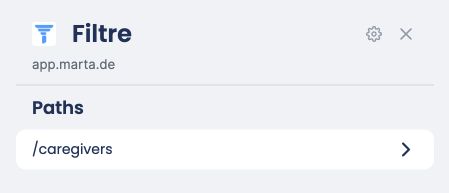
\includegraphics[width=0.7\textwidth]{assets/Filtre_known_paths.png}
  \caption{Screenshot of the known paths page}
  \label{fig:filtreKnownPaths}
\end{figure}

Clicking on one of the items navigates user to a more refined page inside the extension. \autoref{fig:filtreParameters} displays a list of saved URL subpaths and parameters. The user can see the number of times each parameter is called on the right side of the box, as well as when the parameter was last called below the parameter value, on this page. Reloading the page updates the \texttt{lastUpdatedAt} key and the parameter count

Another thing to note is the input field and the "Navigate" button at the bottom of the page. The value in the input field is updated whenever the user navigates through the extension's "directory path" and selects the parameters. By clicking the "Navigate" button, the user can then navigate to the updated URL in a new tab.

\begin{figure}[H]
  \centering
  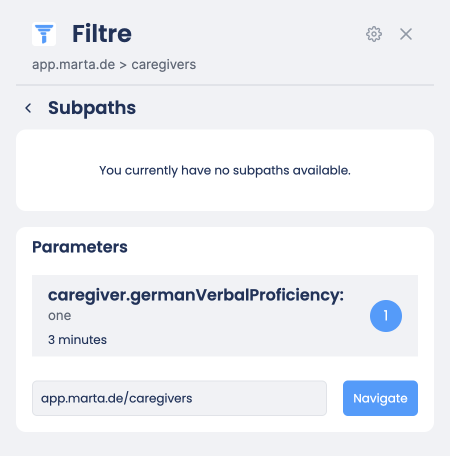
\includegraphics[width=0.7\textwidth]{assets/Filtre_parameters.png}
  \caption{Screenshot of the known subpaths and parameters page}
  \label{fig:filtreParameters}
\end{figure}

With the help of \emph{Storage Area Explorer}\footnote{\emph{Storage Area Explorer} is a simple editor for Storage Area for Chrome Packaged Apps \& Extensions. GitHub repository: \url{https://github.com/jusio/storage-area-explorer}}, it is possible edit or view the \texttt{chrome.storage} using a user interface without the need for console logging the \texttt{chrome.storage} object in the code (See \autoref{fig:storageAreaExplorer}). The current size and size limit are also displayed within the Storage Explorer.

\begin{figure}[H]
  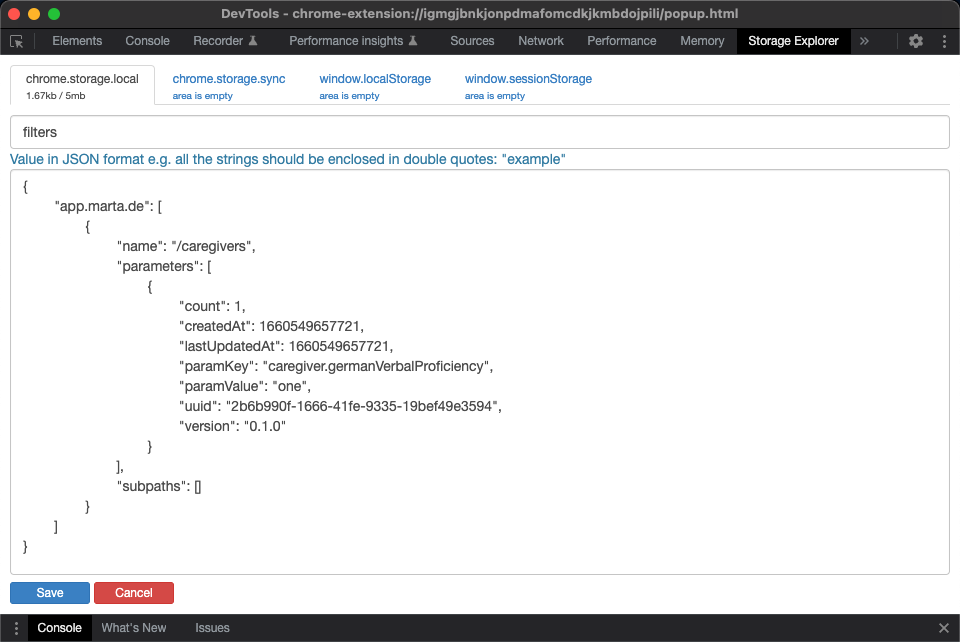
\includegraphics[width=\textwidth]{assets/Storage_area_explorer.png}
  \caption{Screenshot of the Storage Area Explorer}
  \label{fig:storageAreaExplorer}
\end{figure}

\section{Evaluation}
Completion of the goals and criteria described in the requirement analysis should be evaluated as a measure to determine whether the system and its functionalities have achieved their main goal in accordance with the thesis goal. \autoref{table:evaluationTableRequirementAnalysis} shows, sorted by requirement identifier, how far the defined requirements have been implemented:

\begin{tabularx}{\textwidth}{p{0.1\textwidth} p{0.2\textwidth} p{0.6\textwidth}}
  \caption{Evaluation table of requirement analysis}                                                                                                                                                                                                                   \\
  \toprule
  \textbf{ID} & \textbf{Implemented} & \textbf{Remark}                                                                                                                                                                                                                 \\
  \midrule
  FR-01       & \Checkedbox          &                                                                                                                                                                                                                                 \\
  \midrule
  FR-02       & \Checkedbox          & Based on the user's history after installing the extension.                                                                                                                                                                     \\
  \midrule
  FR-03       & \Checkedbox          & It is possible to select multiple parameters. When two identical keys with different values are selected, the second value overwrites the first and no duplicates are produced.                                                 \\
  \midrule
  FR-04       & \Checkedbox          &                                                                                                                                                                                                                                 \\
  \midrule
  FR-05       & \Checkedbox          &                                                                                                                                                                                                                                 \\
  \midrule
  FR-06       & (\Checkedbox)        & The URL is saved but not on each page load because most front-end frameworks nowadays avoid reloading the entire page when navigating through the website. As a result, the URL is now saved whenever the URL value is changed. \\
  \midrule
  FR-07       & \Checkedbox          &                                                                                                                                                                                                                                 \\
  \midrule
  FR-08       & \HollowBox           &                                                                                                                                                                                                                                 \\
  \midrule
  FR-09       & \Checkedbox          & The Clear All Filter button will prompt the user to type "yes" to ensure that the button is not accidentally clicked. To avoid confusion, the button should be differentiated more.                                             \\
  \midrule
  FR-10       & \HollowBox           & Reset configuration button is for now not necessary because currently the only available configuration options are "Excluded Parameters".                                                                                       \\
  \midrule
  NFR-01      & \Checkedbox          &                                                                                                                                                                                                                                 \\
  \midrule
  NFR-02      & \Checkedbox          &                                                                                                                                                                                                                                 \\
  \midrule
  NFR-03      & \Checkedbox          &                                                                                                                                                                                                                                 \\
  \midrule
  NFR-04      & \Checkedbox          &                                                                                                                                                                                                                                 \\
  \midrule
  NFR-05      & \Checkedbox          &                                                                                                                                                                                                                                 \\
  \midrule
  NFR-06      & \Checkedbox          &                                                                                                                                                                                                                                 \\
  \midrule
  NFR-07      & \Checkedbox          &                                                                                                                                                                                                                                 \\
  \bottomrule
  \label{table:evaluationTableRequirementAnalysis}
\end{tabularx}

\noindent With minor exceptions, the extension was thus fully implemented. Usability tests were not carried out.

\section{Publish in the Chrome Web Store}
Releasing the extension in the Chrome Web Store would mean that at least Google can analyze the implementation and identify possible vulnerabilities. However, an internationalization of the extension should be carried out beforehand.
